\section{Discussion about Existing Methods}
% \begin{figure*}[h]
%     \centering
%     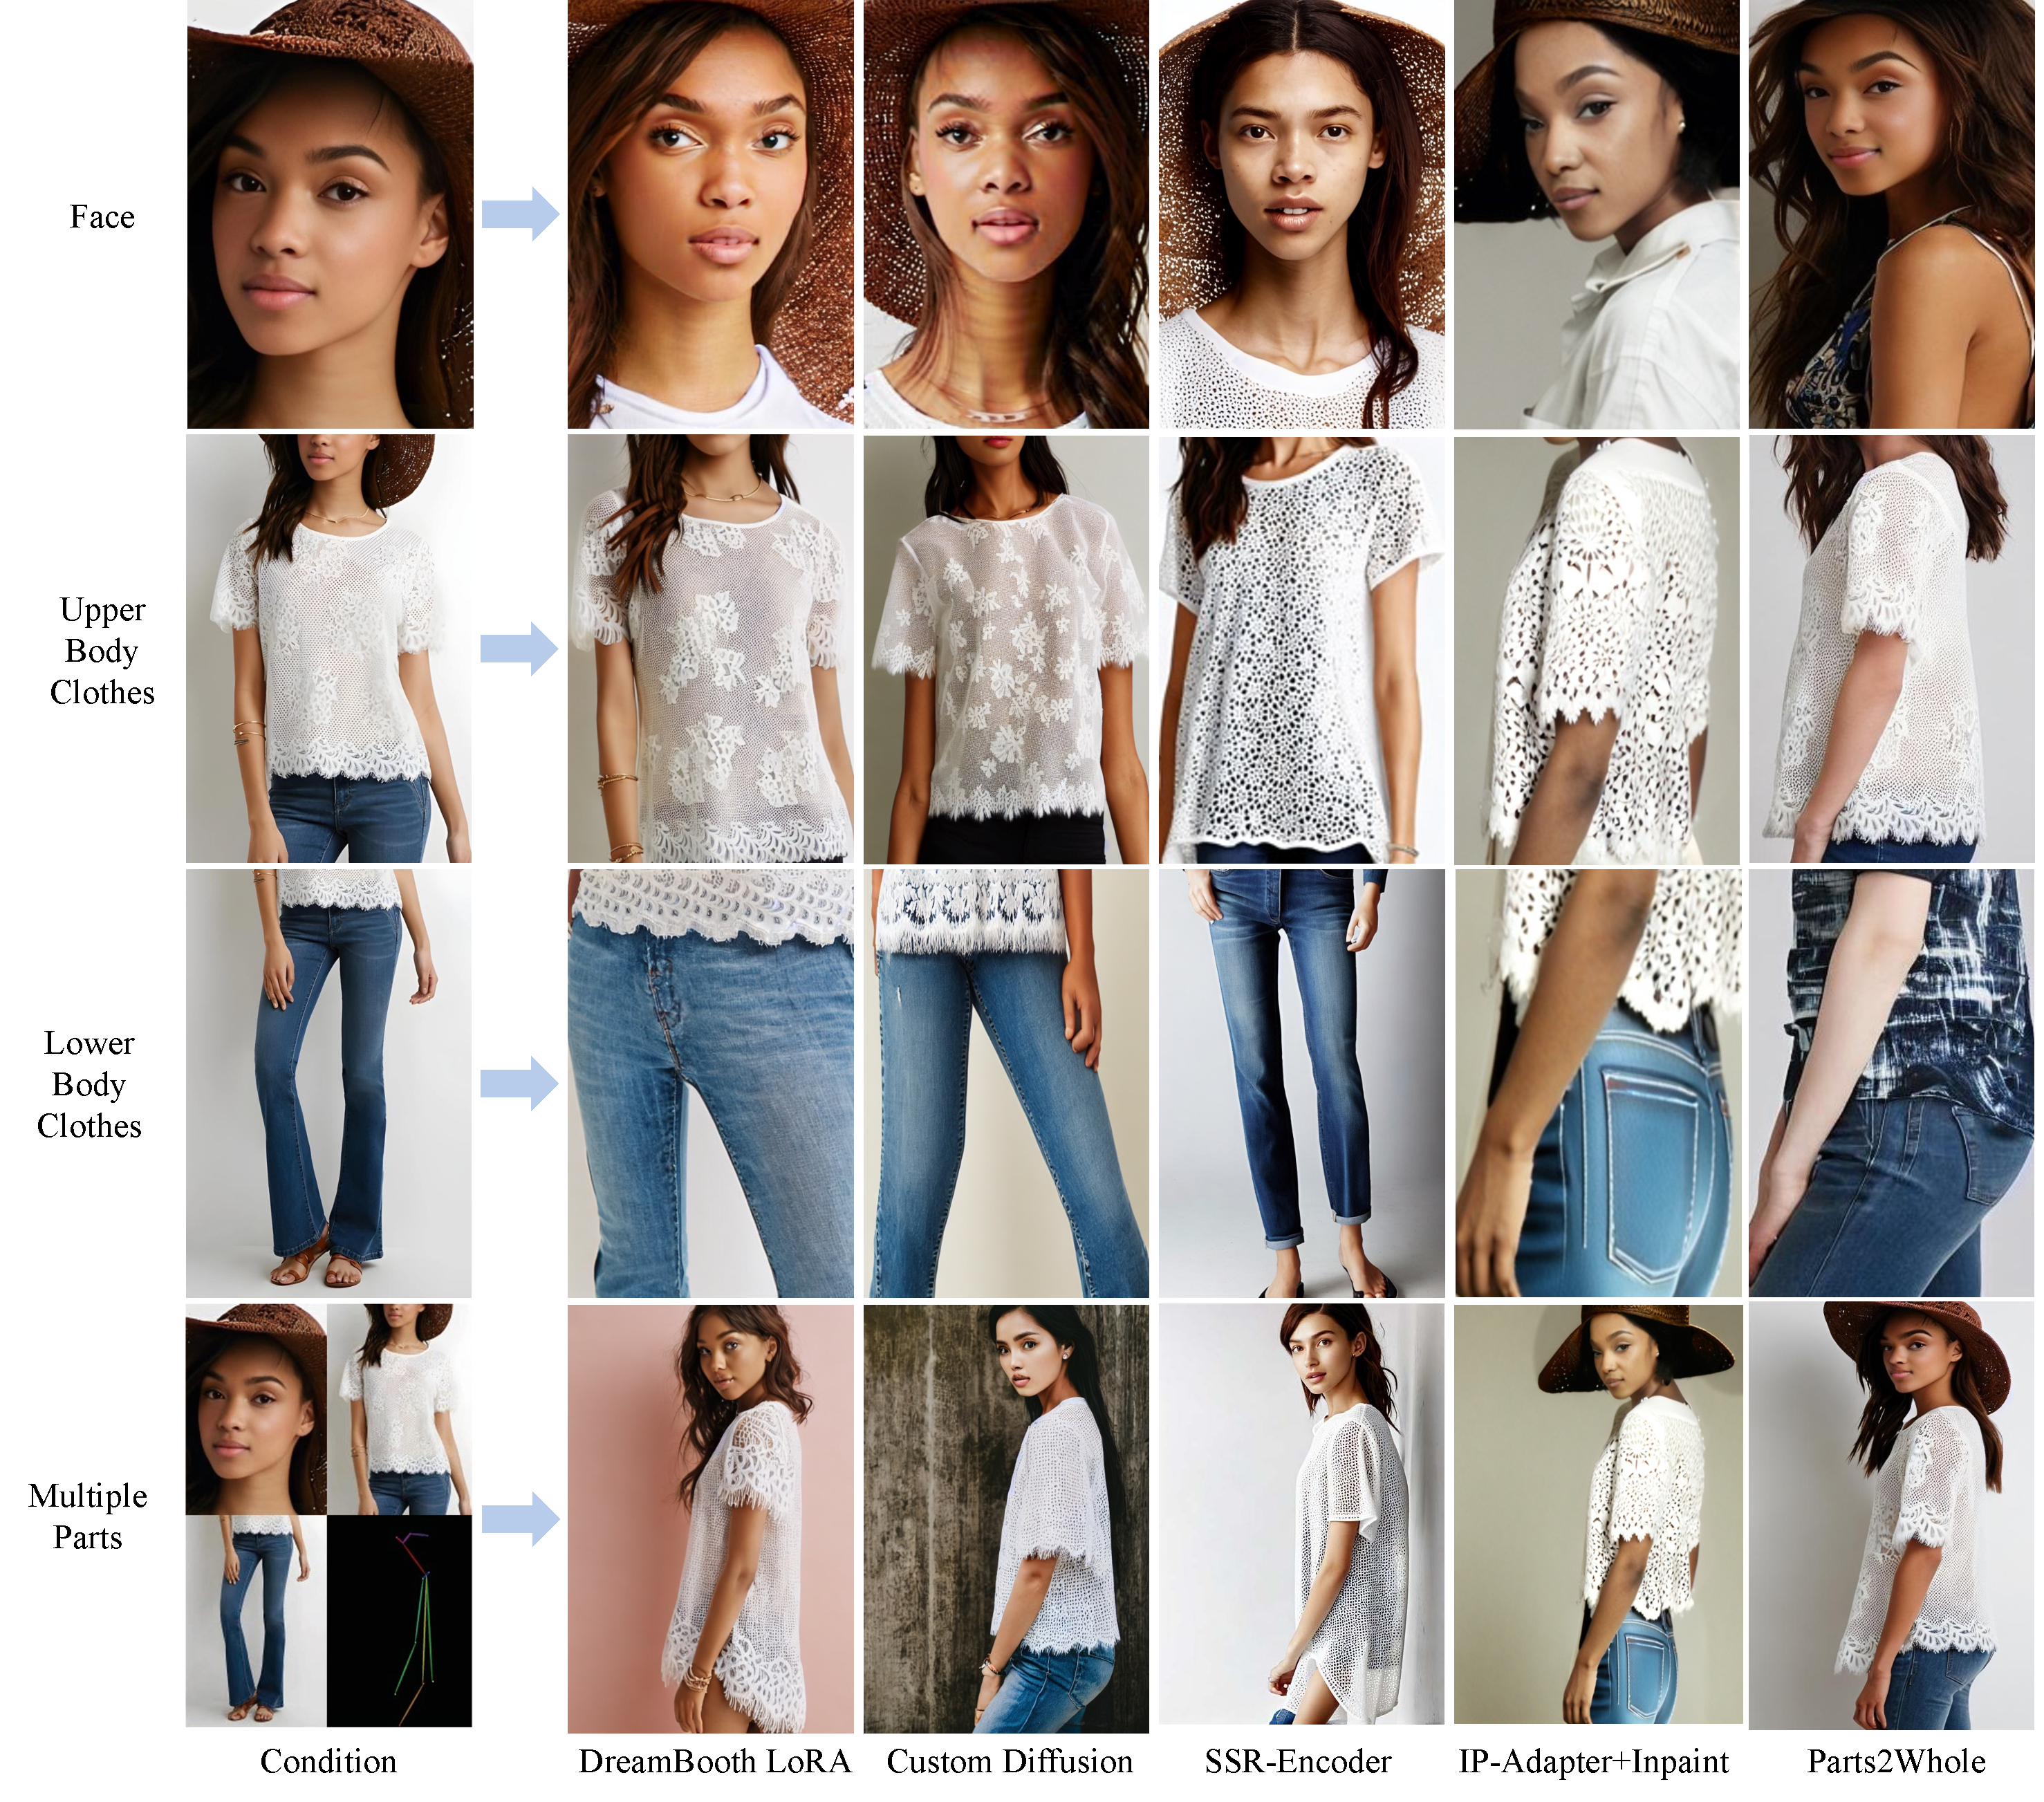
\includegraphics[width=0.9\textwidth]{figure/supp_existing_work.pdf}
%     \caption{Results of single-condition and multi-condition generation. The top three rows labeled "face," "upper body clothes," and "lower body clothes" represent separate control conditions. The fourth row demonstrates joint control under multi-part conditions.}
%     \label{fig:existing_methods}
% \end{figure*}



In our main text, we conduct experiments with both tuning-based methods DreamBooth LoRA~\cite{ruiz2023dreambooth,hu2021lora} and Custom Diffusion~\cite{kumari2023customdiffusion} and tuning-free methods such as IP-Adapter~\cite{ye2023ipadapter} and SSR-Encoder~\cite{zhang2024ssrencoder}. The results of these experiments are further illustrated in Fig~\ref{fig:existing_methods}, which showcases the performance of these methods conditioned on both a single image and multiple images.

The results demonstrate that while these methods generally perform well under a single control condition, they exhibit significant issues when multiple conditions are applied. For example, DreamBooth LoRA encountered cases where pants were omitted, and both Custom Diffusion and SSR-Encoder show alterations in facial ID. The phenomenon observed is attributed to the spatial misalignment of the input multi-body parts with the target image, and the lack of specific design in existing methods to address the variation in spatial positions during feature injection. For instance, methods like SSR-Encoder, Custom Diffusion, and IP-Adapter incorporate features into the denoising UNet through cross-attention mechanisms. They encode reference images into other modal features (e.g. semantic features) and utilize the cross-attention keys ($K$) and values ($V$) from them rather than from \textbf{image dimensional} feature maps. In this process, the correlation between the reference images and the target image \textbf{loses the spatial relationship} of the original image dimensions. It is difficult for these methods to effectively model the attention from various conditional feature maps at different locations in the target image, resulting in a mixture of attributes from different subjects.

Conversely, our Parts2Whole model employs shared self-attention between the reference features and the feature maps in the Denoising U-Net, executed on the image dimension. This allows our model to establish a more precise correlation between different condition images and distinct positions within the feature maps, thereby generating results that are consistent with the detailed attributes of multi-condition images.

% The above mentioned work primarily focuses on image generation under single condition. To further validate the efficacy of our proposed shared self-attention across image dimensional feature maps, we conduct a comparative experiment with the multi-condition generation method UniControl~\cite{qin2023unicontrol}. 
% %The UniControl method does not align spatial positions, and the multi-condition features are directly added to the target feature map. This approach is suitable for multiple spatial relationships are aligned, but not suitable for situations where these relationships vary or are unaligned. 
% The unified controllable generation ability of UniControl relies on amixture of expert (MOE)-style adapter and a task-aware HyperNet .The MoE-style adapter can learn  feature maps from various visual conditions. Meanwhile, the task-aware HyperNet processes task instructions in the form of text prompts, generating embeddings that are task-specific. These embeddings are subsequently integrated into ControlNet to enable precise modulation tailored to distinct visual conditions associated with each task.
% Additionally, the UniControl employs the injection mechanism of ControlNet, which incorporates encoded reference features into the feature maps of UNet. This approach is effective when the condition image and target image structures are aligned. However, due to lack of modeling of spatial position correlation, it is difficult to apply to tasks where multiple condition images are distributed at different locations in the target image.
% The experimental results, shown in \todo{Fig~\ref{fig:existing_methods}}, further substantiate the rationale and efficiency of our shared self-attention mechanism in the task of generating human images from multi-part images. 
